% Created 2020-06-14 Sun 11:02
% Intended LaTeX compiler: pdflatex
\documentclass[dvipdfmx,a4j,14pt,uplatex,openany]{jsbook}
\usepackage[utf8]{inputenc}
\usepackage[T1]{fontenc}
\usepackage{graphicx}
\usepackage{grffile}
\usepackage{longtable}
\usepackage{wrapfig}
\usepackage{rotating}
\usepackage[normalem]{ulem}
\usepackage{amsmath}
\usepackage{textcomp}
\usepackage{amssymb}
\usepackage{capt-of}
\usepackage{hyperref}
\usepackage{coco-jsbook}
\FileVersion{1.0}
\CopyrightAuthor{島野善雄}
\CopyrightYear{2019}
\ConfidentialLevel{機密情報ではない}
\author{Yoshio Shimano}
\date{\textit{[2019-03-30 Sat]}}
\title{ox-Hugo を使う}
\hypersetup{
   bookmarks=true,
   bookmarksnumbered=true,
   colorlinks=true,
   setpagesize=false,
   linkcolor=blue,
   citecolor=blue,
   backref,
   pdfauthor={Yoshio Shimano},
   pdftitle={ox-Hugo を使う},
   pdfkeywords={},
   pdfsubject={Org-mode の中から Hugo を使う方法です。},
   pdfcreator={Emacs 26.3 (Org mode 9.3.7)}, 
   pdflang={Ja}}
  \begin{document}

\maketitle
\color{Black!95!White}

\chapter{はじめに}
\label{sec:orgcfdd19e}
\section{なぜ Hugo を使うのか?}
\label{sec:org757c626}
\begin{quote}
早い!
\end{quote}

の一言につきます。
ポストが少ないのであれば、 Hugo のサイトのリビルドは一瞬です。



\section{なぜ ox-hugo を使うのか?}
\label{sec:orgbfd9aef}
ox-hugo は Org mode から Markdown へのエクスポートバックエンドです。

Hugo は Markdown で書くのが普通ですが、私は Markdown に慣れることが
できません。そこで、 ox-hugo というパッケージを使って、
Org-mode のファイルを Markdown に変換しています。
この ox-hugo というパッケージがなかなか優れもので、
やりたいことはほとんどできます。

それでも、自分の好みの機能がないので、 ox-hugo をカスタマイズして
使っています。uh

\chapter{Hugo のインストール方法}
\label{sec:org82b8f56}
\section{golang のインストール}
\label{sec:org36a47fd}
Hugo は go 言語で動きます。
最初に go 言語をインストールします。

\begin{itemize}
\item \href{https://github.com/golang/go/wiki/Ubuntu}{Ubuntu · golang/go Wiki}
\end{itemize}

を参考にしました。最新のバージョンをインストールするため、
PPA を使います。

\begin{programlist}[label={nil}]{shell}{: }sudo add-apt-repository ppa:gophers/archive
sudo apt update
sudo apt install golang-1.11-go
\end{programlist}

しかしこの方法だと、バイナリが /usr/lib/go-1.11/bin の中にはいってしまいます。

そこで snap を使います:

\begin{programlist}[label={nil}]{shell}{: }sudo snap install --classic go
\end{programlist}

/snap/bin にはいります。

\begin{programlist}[label={nil}]{shell}{: }/snap/bin/go version
\end{programlist}


\section{hugo のインストール}
\label{sec:org6cbd80c}
go 言語がインストールされたら、 hugo をインストールします。


\begin{programlist}[label={nil}]{shell}{: }export GOPATH=$HOME/go
go get -u -v github.com/spf13/hugo
\end{programlist}

\begin{programlist}[label={nil}]{shell}{: }hugo version
\end{programlist}

\chapter{ox-hugo でのプリアンブルの設定方法}
\label{sec:orgc1b71ea}
\begin{programlist}[label={nil}]{text}{: }#+OPTIONS: H:6 num:t
\end{programlist}

\begin{description}
\item[{H:6}] 見出しのレベルを 6 まで出力します。
\item[{num::t}] 見出しに番号をつけます。
\end{description}
\chapter{このサイトでで使える記法}
\label{sec:orgd2ae0ab}
\section{図}
\label{sec:org1d626ef}
これは:

\begin{programlist}[label={nil}]{text}{: }#+ATTR_HTML: :alt test :width 25%
#+caption: Reddit Icon
[[file:images/Org-mode-unicorn.svg]]
\end{programlist}

次に変換されます:

\begin{figure}{p}
\centering
\includesvg[width=0.5\textwidth]{images/Org-mode-unicorn}
\caption{Reddit Icon}
\end{figure}


\newpage

\section{Babel}
\label{sec:orge96a5d2}
Org-mode の中でプログラミング言語を書くことができます。
それだけではなく、 Org-mode の中でプログラムを実行することが
できます。

この Ditaa のプログラムは:

\begin{center}
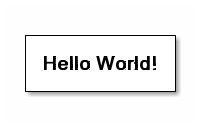
\includegraphics[width=.7\linewidth]{hello-world.png}
\end{center}

このように変換されます:

\begin{figure}{h}
\centering
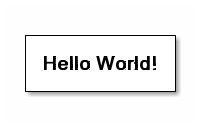
\includegraphics[width=0.5\textwidth]{hello-world.png}
\caption{\label{fig:first}Ditaa の出力}
\end{figure}


\section{数式}
\label{sec:org76ed477}
\subsection{インライン数式}
\label{sec:org51cf58a}
例えば下の Org mode の断片は:

\begin{programlist}[label={nil}]{text}{: }LaTeX formatted equation: \( E = -J \sum_{i=1}^N s_i s_{i+1} \)
\end{programlist}

これは Hugo がレンダリングする HTML の中でこのように見えます:

\LaTeX{} formatted equation: \(E = -J \sum_{i=1}^N s_i s_{i+1 }\)
\subsection{\LaTeX の数式}
\label{sec:org2f4c1d0}
\texttt{ox-hugo} は \LaTeX の環境をサポートしています。

下の Org mode の断片は:

\begin{programlist}[label={latex-example}]{text}{: }\begin{equation}
\label{eq:0}
C = W\log_{2} (1+\mathrm{SNR})
\end{equation}
\end{programlist}

次のようにエクスポートされます:

\begin{equation}
\label{eq:1}
C = W\log_{2} (1+\mathrm{SNR})
\end{equation}

\texttt{\textbackslash{}ref\{eq:1\}} は \ref{eq:1} へと変換されます<。



\section{コードブロック}
\label{sec:orge91f4d9}
いくつかのコードの例です:

\begin{programlist}[label={nil}]{lisp}{: }(message "Hello")
\end{programlist}

\begin{programlist}[label={nil}]{shell}{: }ls -al
\end{programlist}


\begin{programlist}[label={nil}]{ruby}{: Ruby の例}print("test")
\end{programlist}

上の Ruby コードの出力です:

\begin{exampleoutput}
test
\end{exampleoutput}


\section{表}
\label{sec:org6b304f1}
\index{table}
これは (\ref{tab:test1}):

\begin{programlist}[label={nil}]{text}{: }#+name: tab:test1
#+caption: 表のテスト
|---+---+---|
| a | b | c |
|---+---+---|
| 1 | 2 | 3 |
| 1 | 2 | 3 |
| 1 | 2 | 3 |
|---+---+---|
\end{programlist}

このように出力されます:

\begin{table}[htbp]
\caption{\label{tab:test1}表のテスト}
\centering
\begin{tabular}{rrr}
\hline
a & b & c\\
\hline
1 & 2 & 3\\
1 & 2 & 3\\
1 & 2 & 3\\
\hline
\end{tabular}
\end{table}

\section{引用}
\label{sec:orgd3ee530}
\subsection{素の quote ブロック}
\label{sec:orgb1fc4bd}
素の quote ブロックの出力です。

\begin{programlist}[label={nil}]{text}{: }#+begin_quote :author Shimano
こんなものですかね。引用は。うまくいきます?
#+end_quote
\end{programlist}

\begin{quote}
こんなものですかね。引用は。うまくいきます?
\end{quote}

\subsection{\texttt{quote} ショートコードを使う}
\label{sec:org496560b}
\subsubsection{\texttt{quote} ショートコード}
\label{sec:org5e79dba}
このような \texttt{quote} ショートコード を作りました。あ

\begin{programlist}[label={nil}]{html}{: }{{- $author := .Get "author" -}}
{{- $width := .Get "width" -}}
<div class="w3-panel w3-card-4 w3-light-grey"
  {{ if eq $width ""}}
     style="width:50%"
  {{ else }}
     style="width:{{$width}}"
  {{ end }}>
  <i class="fa fa-quote-left w3-large w3-text-red"></i><br>
  <p class="w3-large">
    {{ .Inner  }}
  </p>
{{ with $author }}
  <p class="w3-large w3-right">by: {{.}}</p><br>
{{ end }}
<i class="fa fa-quote-right w3-large w3-text-red"></i><br>
</div>
\end{programlist}

\subsubsection{著者ありの例:}
\label{sec:orga22217d}
\begin{programlist}[label={quote-with-authr}]{text}{: 著者ありの引用}#+HTML: {{% blockquote width="30%" author="shimano" %}}
#+begin_quotation :author Shimano
こんなものですかね。引用は。うまくいきます?
#+end_quotation
#+HTML: 
\end{programlist}

これが出力されます:

\begin{quotation}
こんなものですかね。引用は。うまくいきます?
\end{quotation}

\subsubsection{著者なしの例:}
\label{sec:orgbdff6cf}
\begin{programlist}[label={quote-wihtout-author}]{text}{: }#+HTML: {{% blockquote width="70%" %}}
#+begin_quotation :author Shimano
こんなものですかね。引用は。うまくいきます?
#+end_quotation
#+HTML: 
\end{programlist}

これが出力されます:

\begin{quotation}
こんなものですかね。引用は。うまくいきます?
\end{quotation}

\section{スペシャルブロック}
\label{sec:org40f1366}
Org-mode の中のスペシャルブロックは \texttt{<div>} へ変換されます。
クラスを設定するには、 \texttt{\#+ATTR\_HTML: :class} を設定します。 

この Org-mode のスペシャルブロックは:

\begin{programlist}[label={nil}]{text}{: }#+ATTR_HTML: :class w3-panel w3-blue w3-border
#+begin_info
Info 

This is a test.
#+end_info
\end{programlist}

これへと変換されます:

\begin{info}
Info 

This is a test.
\end{info}

\begin{programlist}[label={nil}]{text}{: }#+ATTR_HTML: :class w3-panel w3-yellow w3-border
#+begin_info
#+begin_warning
Warning

This is a test.
#+end_warning
\end{programlist}

\begin{warning}
Warning

This is a test.
\end{warning}

\section{例のブロック}
\label{sec:orgb093244}
\begin{programlist}[label={nil}]{ruby}{: }p "test"
\end{programlist}
\end{document}